\documentclass[11pt,a4paper]{article}
\usepackage[spanish,es-nodecimaldot]{babel}	% Utilizar español
\usepackage[utf8]{inputenc}					% Caracteres UTF-8
\usepackage{graphicx}						% Imagenes
\usepackage[hidelinks]{hyperref}			% Poner enlaces sin marcarlos en rojo
\usepackage{fancyhdr}						% Modificar encabezados y pies de pagina
\usepackage{float}							% Insertar figuras
\usepackage[textwidth=390pt]{geometry}		% Anchura de la pagina
\usepackage[nottoc]{tocbibind}				% Referencias (no incluir num pagina indice en Indice)
\usepackage{enumitem}						% Permitir enumerate con distintos simbolos
\usepackage[T1]{fontenc}					% Usar textsc en sections
\usepackage{amsmath}						% Símbolos matemáticos
\usepackage{xlop}

% Comando para poner el nombre de la asignatura
\newcommand{\asignatura}{Arquitectura y Computación de Altas Prestaciones}
\newcommand{\autor}{Vladislav Nikolov Vasilev}
\newcommand{\titulo}{Trabajo de Teoría}
\newcommand{\subtitulo}{Ejercicio de redes de interconexión}
\newcommand{\rama}{Ingeniería de Computadores}

% Configuracion de encabezados y pies de pagina
\pagestyle{fancy}
\lhead{\autor{}}
\rhead{\asignatura{}}
\lfoot{Grado en Ingeniería Informática}
\cfoot{}
\rfoot{\thepage}
\renewcommand{\headrulewidth}{0.4pt}		% Linea cabeza de pagina
\renewcommand{\footrulewidth}{0.4pt}		% Linea pie de pagina

\begin{document}
\pagenumbering{gobble}

% Pagina de titulo
\begin{titlepage}

\begin{minipage}{\textwidth}

\centering

%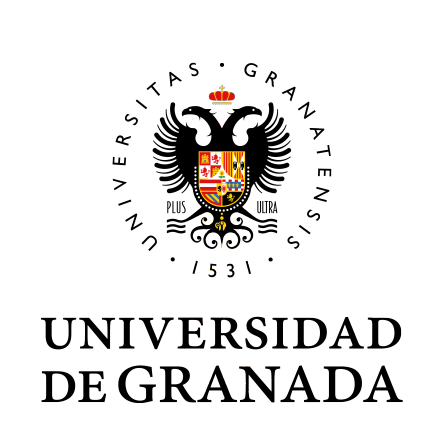
\includegraphics[scale=0.5]{img/ugr.png}\\

\includegraphics[scale=0.3]{img/logo_ugr.jpg}\\[1cm]

\textsc{\Large \asignatura{}\\[0.2cm]}
\textsc{GRADO EN INGENIERÍA INFORMÁTICA}\\[1cm]

\noindent\rule[-1ex]{\textwidth}{1pt}\\[1.5ex]
\textsc{{\Huge \titulo\\[0.5ex]}}
\textsc{{\Large \subtitulo\\}}
\noindent\rule[-1ex]{\textwidth}{2pt}\\[3.5ex]

\end{minipage}

%\vspace{0.5cm}
\vspace{0.7cm}

\begin{minipage}{\textwidth}

\centering

\textbf{Autor}\\ {\autor{}}\\[2.5ex]
\textbf{Rama}\\ {\rama}\\[2.5ex]
\vspace{0.3cm}


\includegraphics[scale=0.3]{img/etsiit.jpeg}

\vspace{0.7cm}
\textsc{Escuela Técnica Superior de Ingenierías Informática y de Telecomunicación}\\
\vspace{1cm}
\textsc{Curso 2019-2020}
\end{minipage}
\end{titlepage}

\pagenumbering{arabic}

\setlength{\parskip}{1em}

\noindent
\textbf{Imaginemos un multiprocesador de memoria distribuida con red de interconexión toro
bidimensional, canales bidireccionales y 1024 nodos terminales (supongamos igual base en las dos
dimensiones).
Los conmutadores de la red tienen buffers asociados solo a la entrada. Esto hace que en las
técnicas de conmutación que aprovechan para la transferencia la segmentación en etapas del camino
por parte de los buffers, se tenga que tener en cuenta, al obtener la latencia de transporte que
todas las etapas de conmutación incluyen atravesar un conmutador y el canal que lo une al
siguiente conmutador o al interfaz de red correspondiente. Los tiempos que determinan el retardo
de comunicación en el sistema de comunicación son: $t_{sobrecarga_o} = 2\mu s$ (tiempo de sobrecarga
en el origen). $t_{sobrecarga_d} = 2\mu s$ (tiempo de sobrecarga en el destino). $t_r = 3 ns$ (tiempo
requerido por el algoritmo de encaminamiento en el conmutador); $t_w = 6 ns$ (tiempo de
transferencia de 1 phit entre conmutadores);}

\noindent
\textbf{Supongamos un paquete de 126 phits + 2 phits de cabecera.}

\noindent
\textbf{Calcular la latencia (téngase en cuenta también la sobrecarga) que supone la transferencia de este paquete desde el nodo 752 al nodo 27 por el camino más corto, Si se utiliza conmutación de circuitos con camino segmentado (consideramos que un flit y un phit tienen el mismo tamaño, y que la sonda y el reconocimiento ocupa 1 flit).
}

\textbf{Solución}

Sabemos que la red es un toro bidimensional con 1024 nodos terminales y que las dos dimensiones
tienen igual base. Esto significa que el valor de la base es 32, ya que $32 = 2^5$, y tenemos
que $2^5 \cdot 2^5 = 2^{10} = 1024$.

Ahora, lo primero que tenemos que hacer es pasar las coordenadas de los nodos origen y destino
a base 32. Tenemos lo siguiente:

\begin{minipage}{\textwidth}
  \centering
  $\opidiv{752}{32}$\qquad\qquad\qquad$\opidiv{27}{32}$
\end{minipage}

\begin{itemize}
	\item Nodo origen: $752 = 23, 16_{)32}$
	\item Nodo destino: $27 = 0, 27_{)32}$
\end{itemize}

Ahora, tenemos que calcular la distancia entre los dos nodos. Al ser la rodo un toro
bidimensional, tenemos que calcular la distancia del nodo origen al destino y del destino al
origen, y nos quedamos con las distancias mínimas en cada dimensión:

$$dist(\text{Origen, Destino}) = 0-23,  27-16_{)32} = -23, 11_{)32} = 9, 11_{)32}$$

$$dist(\text{Destino, Origen}) = 23-0,  16-27_{)32} = 23, -11_{)32} = 23, 21_{)32}$$

$$dist\_min(752, 27) = 9 + 11 = 20$$

Ahora tenemos que calcular $D$, que es el número de parejas \textit{switch}-enlace. El valor de
$D$ es el siguiente:

$$D = dist\_min + 1 = 20 + 1 = 21$$

Con estos datos, vamos a calcular el tiempo de conmutación, $t_{CC}$. El tiempo de
conmutación es la suma del tiempo de sonda, el tiempo de reconocimiento y el tiempo de datos.
La expresión es la siguiente:

$$t_{CC} = t_{sonda} + t_{reconocimiento} + t_{datos}$$

Vamos a calcular primero el tiempo de sonda. La sonda tiene un tamaño de 1 flit. Por tanto,
vamos a enviar 1 flit de la cabecera, y vamos a enviar el otro después de recibir el
reconocimiento. A la hora de calcular los tiempos, \textbf{vamos a tener en cuenta el tiempo
que se tarda en enviar la información de la tarjeta de red del origen al primer conmutador}.
A continuación se puede ver el tiempo de sonda:

\begin{equation}
\begin{split}
t_{sonda} &= 1\;phit \times t_w + D(t_r + 1\;phit \times t_w) \\
& = 1\;phit \times 6\text{ns}/phit + 21(3ns + 1\;phit \times 6\text{ns}/phit) \\
&= 6\text{ns} + 21 \times 9\text{ns} = 6\text{ns} + 189\text{ns} = \mathbf{195}\textbf{\text{ns}}
\end{split}
\end{equation}

Ahora calculemos el tiempo de reconocimiento:

\begin{equation}
\begin{split}
t_{reconocimiento} &= D(t_r + 1\;phit \times t_w) + 1\;phit \times t_w\\
& = 21(1\;phit \times 6\text{ns}/phit) + 1\;phit \times 6\text{ns}/phit \\
&= 21 \times 6\text{ns} + 6\text{ns} = 126\text{ns} + 6\text{ns} = \mathbf{132}\textbf{\text{ns}}
\end{split}
\end{equation}

Y finalmente, el tiempo de datos. Anteriormente enviamos 1 flit de los 128 flits del paquete.
Por tanto, \textbf{nos quedan por enviar que enviar 127 flits}. Como los datos son enviados
por el camino segmentado, el tiempo que tardarán en llegar todos vendrá dado por el tiempo
que tarda en llegar el primer flit más lo que tarden en atravesar la última etapa del camino
segmentado los 126 flits restantes. Este úlitmo tiempo viene dado por el tiempo de transferencia
entre conmutadores, $t_w$. A continuación se puede ver el resultado:

\begin{equation}
\begin{split}
t_{datos} &= 1\;phit \times t_w + D(1\;phit \times t_w) + 126\;phit \times t_w\\
& = 1\;phit \times 6\text{ns}/phit + 21(1\;phit \times 6\text{ns}/phit) + 126\;phit \times 6\text{ns}/phit \\
&= 6\text{ns} + 21 \times 6\text{ns} + 756\text{ns} = 6\text{ns} + 126\text{ns} + 756\text{ns} = \mathbf{888}\textbf{\text{ns}}
\end{split}
\end{equation}

El tiempo total de conmutación es el siguiente:

\begin{equation}
\begin{split}
t_{CC} &= t_{sonda} + t_{reconocimiento} + t_{datos} = 195\text{ns} + 132\text{ns} + 888\text{ns}
\\
&= 1215\text{ns} = \mathbf{1.215\mu}\text{s}
\end{split}
\end{equation}

La latencia viene dada por el tiempo de conmutación y los tiempos de sobrecarga en el nodo
origen y en el nodo destino. Por tanto, la latencia ($T_{CC}$) tiene el siguiente valor:

\begin{equation}
\begin{split}
T_{CC} &= t_{CC} + t_{sobrecarga_o} + t_{sobrecarga_d} = 1.215\mu \text{s} + 2\mu \text{s} + 2\mu \text{s} \\
&= \mathbf{5.215\mu}\text{s}
\end{split}
\end{equation}

\end{document}

